\documentclass[xcolor=x11names, aspectratio=169,usenames,dvipsnames]{beamer}
\usepackage[british]{babel}
\usepackage{amsmath}
\usepackage{amssymb}
\usepackage{amsfonts}
\usepackage{mathpazo}
\usepackage{enumerate}
\usepackage{array,booktabs}
\usepackage{tikz}
\usepackage{mathdots}
\usepackage{verbatim}
\usepackage{multirow}
\usepackage{tabularx}
\usetikzlibrary{shadows,matrix,backgrounds,patterns,arrows,decorations.markings,shapes,positioning,calc,chains,scopes,fit}
\usepackage{caption}

\usetheme[titleformat title=regular,titleformat frame=regular,titleformat section=allcaps,numbering=fraction]{metropolis}

\author[T.\ Evans \&\ F.\ Kußmaul]{\large Tim Evans\inst{1}, \and Felix Kußmaul\inst{2}}
\title[Mining Paper Catalogues]{\Large Mining Paper Catalogues}
\subtitle{\normalsize A Multilingual Solution to Reduce Verbose Fields to Consistent Terminology}
\institute[York, Cologne]{\inst{1} Archaeology Data Service, University of York \and \inst{2} Archaeological Institute, University of Cologne}
\date[31 August 2017]{\vspace*{1em}23rd Annual Meeting EAA, Maastricht\\[.5em] 31 August 2017\vspace*{1em}}

\titlegraphic{
    \tikz[overlay,remember picture]
        \node[xshift=-5em,yshift=3em,at=(current page.south east), anchor=south east] {
            
\includegraphics[width=0.25\textwidth]{img/archaide.eps}
        };
}
\usepackage{pdfrender}

\newcommand{\red}[1]{\textcolor{red}{#1}}
\newcommand{\orange}[1]{\textcolor{orange}{#1}}
\newcommand{\green}[1]{\textcolor{markgreen}{#1}}
\newcommand{\textgreen}[1]{\textcolor{textgreen}{#1}}
\newcommand{\blue}[1]{\textcolor{textblue}{#1}}
\newcommand{\gray}[1]{\textcolor{gray}{#1}}

\newcolumntype{R}{>{\centering\raggedleft\arraybackslash}X}
\newcolumntype{L}{>{\centering\raggedright\arraybackslash}X}
\newcolumntype{C}{>{\centering\arraybackslash}X}

\usepackage[style=authortitle-comp,backend=biber]{biblatex}
\addbibresource{eaa.bib}
\renewcommand*{\bibfont}{\small}

\setbeamercovered{transparent}

\newcommand{\textsb}[1]{{\fontfamily{cmss}\fontseries{sbc}\fontshape{n}\selectfont #1}}

\setbeamertemplate{enumerate items}[square]

\setbeamertemplate{footline}
{
\hbox{%
  \begin{beamercolorbox}[wd=.26\paperwidth,ht=2.7ex,dp=1.2ex,center]{author in head/foot}%
    \usebeamerfont{author in head/foot}\insertshortauthor\ (\insertshortinstitute)
  \end{beamercolorbox}%
  \begin{beamercolorbox}[wd=.40\paperwidth,ht=2.7ex,dp=1.2ex,center]{author in head/foot}%
    \usebeamerfont{title in head/foot}\insertshorttitle:\ \textbf{\insertsection}
  \end{beamercolorbox}%
  \begin{beamercolorbox}[wd=.36\paperwidth,ht=2.7ex,dp=1.2ex,center]{author in head/foot}%
    \usebeamerfont{date in head/foot}\insertshortdate\hfill\insertframenumber/\inserttotalframenumber\strut
  \end{beamercolorbox}}
  \vskip0pt%
}

\tikzset{
  invisible/.style={opacity=0},
  visible on/.style={alt={#1{}{invisible}}},
  alt/.code args={<#1>#2#3}{%
    \alt<#1>{\pgfkeysalso{#2}}{\pgfkeysalso{#3}} % \pgfkeysalso doesn't change the path
  },
}

%\newcommand{\printSectionYes}{\AtBeginSection[]
%{
% \begin{frame}{Agenda}
% \tableofcontents[sectionstyle=show/shaded,
% 					subsectionstyle=show/shaded/hide]
% \end{frame}
%}}

\tikzset{onslide/.code args={<#1>#2}{%
  \only<#1>{\pgfkeysalso{#2}}%
}}

\setbeamertemplate{section in toc shaded}[default][50]

\setbeamertemplate{subsection in toc shaded}[default][50]

\makeatletter
\patchcmd{\beamer@sectionintoc}{\vskip1.5em}{\vskip0.5em}{}{}
\makeatother

\makeatletter
\newcommand\footnoteref[1]{\protected@xdef\@thefnmark{\ref{#1}}\@footnotemark}
\makeatother

\setbeamertemplate{bibliography item}{%
  \ifboolexpr{ test {\ifentrytype{book}} or test {\ifentrytype{mvbook}}
    or test {\ifentrytype{collection}} or test {\ifentrytype{mvcollection}}
    or test {\ifentrytype{reference}} or test {\ifentrytype{mvreference}} }
    {\setbeamertemplate{bibliography item}[book]}
    {\ifentrytype{online}
       {\setbeamertemplate{bibliography item}[online]}
       {\setbeamertemplate{bibliography item}[article]}}%
  \usebeamertemplate{bibliography item}}
  
\defbibenvironment{bibliography}
  {\list{}
     {\settowidth{\labelwidth}{\usebeamertemplate{bibliography item}}%
      \setlength{\leftmargin}{\labelwidth}%
      \setlength{\labelsep}{\biblabelsep}%
      \addtolength{\leftmargin}{\labelsep}%
      \setlength{\itemsep}{\bibitemsep}%
      \setlength{\parsep}{\bibparsep}}}
  {\endlist}
  {\item}
  
%%% DEFINE DOCUMENT SHAPE
% taken from manual
\makeatletter
\pgfdeclareshape{document}{
\inheritsavedanchors[from=rectangle] % this is nearly a rectangle
\inheritanchorborder[from=rectangle]
\inheritanchor[from=rectangle]{center}
\inheritanchor[from=rectangle]{north}
\inheritanchor[from=rectangle]{south}
\inheritanchor[from=rectangle]{west}
\inheritanchor[from=rectangle]{east}
% ... and possibly more
\backgroundpath{% this is new
% store lower right in xa/ya and upper right in xb/yb
\southwest \pgf@xa=\pgf@x \pgf@ya=\pgf@y
\northeast \pgf@xb=\pgf@x \pgf@yb=\pgf@y
% compute corner of ‘‘flipped page’’
\pgf@xc=\pgf@xb \advance\pgf@xc by-5pt % this should be a parameter
\pgf@yc=\pgf@yb \advance\pgf@yc by-5pt
% construct main path
\pgfpathmoveto{\pgfpoint{\pgf@xa}{\pgf@ya}}
\pgfpathlineto{\pgfpoint{\pgf@xa}{\pgf@yb}}
\pgfpathlineto{\pgfpoint{\pgf@xc}{\pgf@yb}}
\pgfpathlineto{\pgfpoint{\pgf@xb}{\pgf@yc}}
\pgfpathlineto{\pgfpoint{\pgf@xb}{\pgf@ya}}
\pgfpathclose
% add little corner
\pgfpathmoveto{\pgfpoint{\pgf@xc}{\pgf@yb}}
\pgfpathlineto{\pgfpoint{\pgf@xc}{\pgf@yc}}
\pgfpathlineto{\pgfpoint{\pgf@xb}{\pgf@yc}}
\pgfpathlineto{\pgfpoint{\pgf@xc}{\pgf@yc}}
}
}
\makeatother


%\setbeamertemplate{title page}{%
%\begin{tikzpicture}[remember picture,overlay]
%\fill[orange]
%  ([yshift=15pt]current page.west) rectangle (current page.south east);
%\node[anchor=east] 
%  at ([yshift=-50pt]current page.north east) (author)
%  {\parbox[t]{.6\paperwidth}{\raggedleft%
%    \usebeamerfont{author}\textcolor{orange}{%
%    \textpdfrender{
%    TextRenderingMode=FillStroke,
%    FillColor=orange,
%    LineWidth=.1ex,
%    }{\insertauthor}}}};
%\node[anchor=north east] 
%  at ([yshift=-70pt]current page.north east) (institute)
%  {\parbox[t]{.78\paperwidth}{\raggedleft%
%    \usebeamerfont{institute}\textcolor{gray}{\insertinstitute}}};
%\node[anchor=south west] 
%  at ([yshift=20pt]current page.west) (logo)
%  {\parbox[t]{.19\paperwidth}{\raggedleft%
%    \usebeamercolor[fg]{titlegraphic}\inserttitlegraphic}};
%\node[anchor=east]
%  at ([yshift=-10pt,xshift=-20pt]current page.east) (title)
%  {\parbox[t]{\textwidth}{\raggedleft%
% \usebeamerfont{author}\textcolor{white}{%
%    \textpdfrender{
%    TextRenderingMode=FillStroke,
%    FillColor=white,
%    LineWidth=.1ex,
%    }{\inserttitle}}}};
%\node[anchor=east]
%  at ([yshift=-60pt,xshift=-20pt]current page.east) (subtitle)
%  {\parbox[t]{.6\paperwidth}{\raggedleft\usebeamerfont{subtitle}\textcolor{black}{\insertsubtitle}}};
%\end{tikzpicture}
%}
\definecolor{morange}{HTML}{FF8200}
\metroset{block=fill}
 
\begin{document}

\begin{frame}[plain]
\titlepage
\end{frame}

\begin{frame}{Data Source}
\begin{center}
\begin{figure}
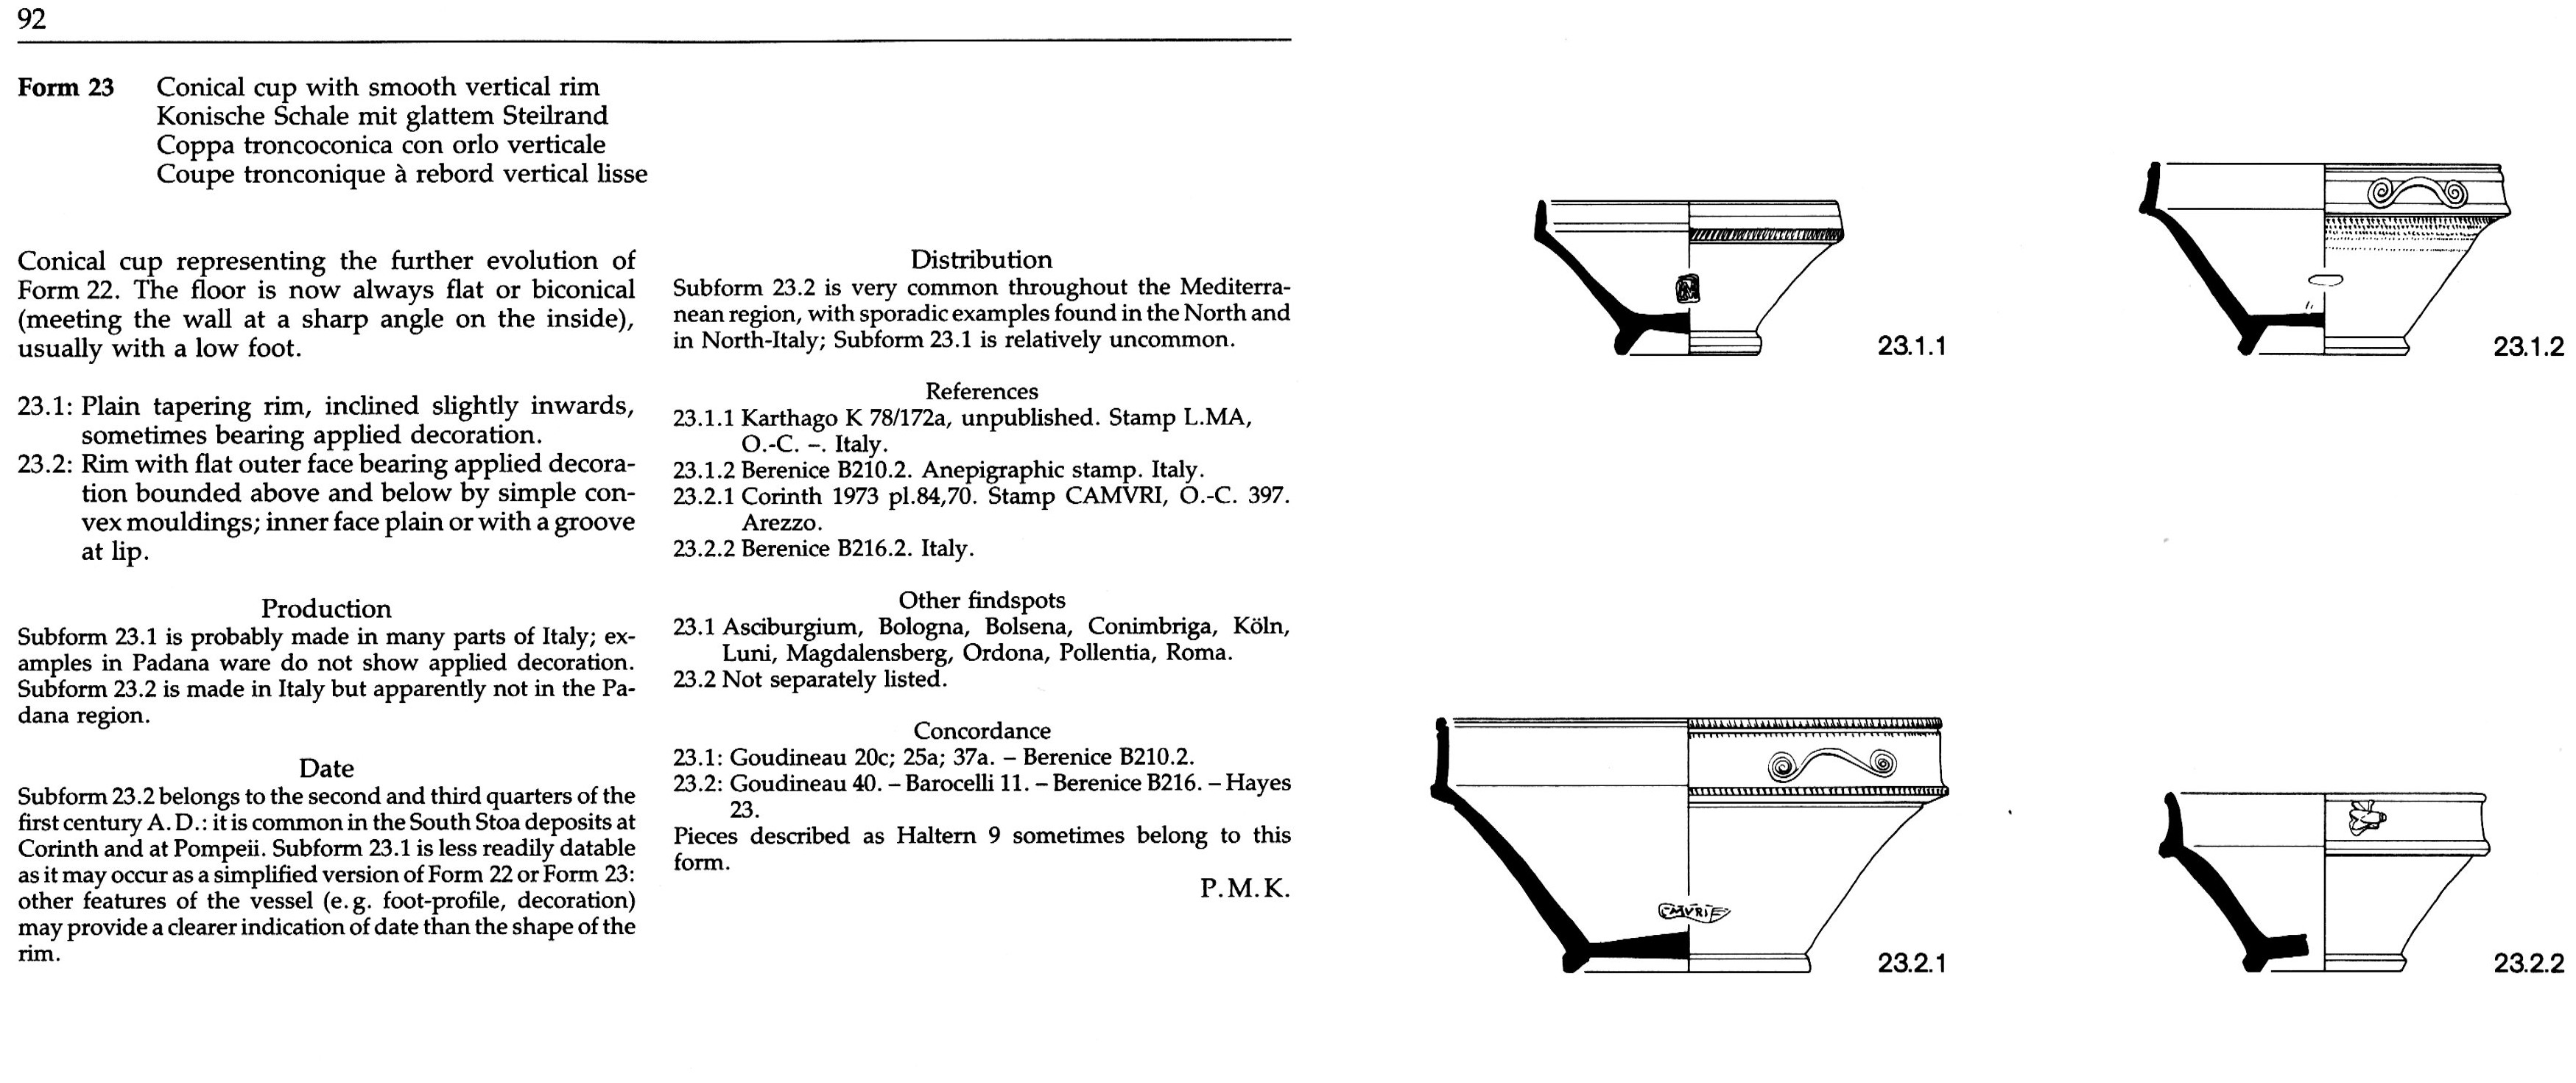
\includegraphics[width=.875\paperwidth]{img/consp.jpg}
\caption{Sample from \cite{consp}.}
\end{figure}
\end{center}
\end{frame}

\begin{frame}{Oh dear!}
\begin{block}{Problem}\vspace{.5em}
Running texts contain a lot of \emph{irrelevant information} (for machine processing).

This makes database lookups without keywords \alert{\textbf{extremely inefficient}}.
\end{block}
\end{frame}

\begin{frame}[fragile]{}
\begin{minipage}[t]{0.45\textwidth}
What we \textbf{have}:\medskip

\begin{figure}
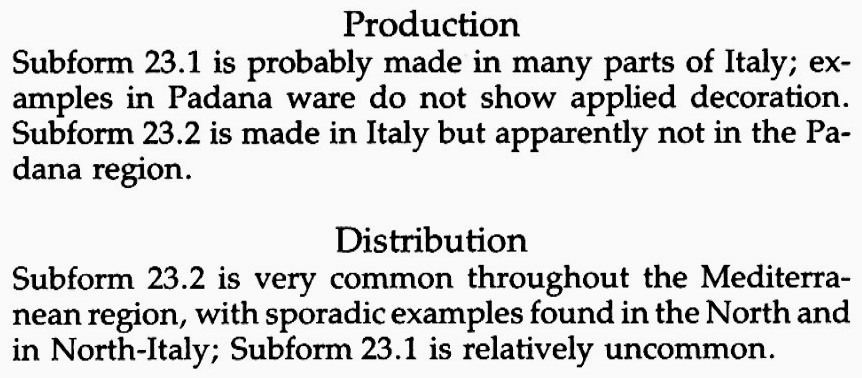
\includegraphics[width=1.0\textwidth]{img/consp_ex.jpg}
\end{figure}
\end{minipage}\hfill\pause
\begin{minipage}[t]{0.45\textwidth}
What we \textbf{want}:\medskip
{\scriptsize
\begin{verbatim}
{
   "form": "23.1",
   "origin": "Italy",
   "decoration": "none",
   "occurs": "uncommon"
},
{
   "form": "23.2",
   "origin": "Italy, not Padana",
   "occurs": "Mediterranean region;
              North-Italy"
}
\end{verbatim}
}
\end{minipage}\pause\medskip

\begin{minipage}[t]{0.45\textwidth}
\begin{center}
\alert{\textbf{UNSTRUCTURED DATA}}
\end{center}
\end{minipage}\hfill
\begin{minipage}[t]{0.45\textwidth}
\begin{center}
\alert{\textbf{STRUCTURED DATA}}
\end{center}
\end{minipage}
\end{frame}

%\begin{frame}{Classification}
%\begin{block}{Definition: Text Mining}\vspace{.5em}
%\textbf{Text Mining} is a \alert{general term} covering several different ideas\pause, e.\,g.:
%\begin{itemize}[<+->]
%\item Statistical analysis
%\item Information retrieval
%\item \textbf{Information extraction}
%\item\dots
%\end{itemize}
%\end{block}
%\end{frame}

\begin{frame}{Information Extraction}
\begin{block}{Definition: Information Extraction (IE)}\vspace{.5em}{
\enquote{\textit{[\textbf{IE} refers to] the \textbf{identification} and extraction of instances of a particular class of events or relationships in a \textbf{natural language text} and their \textbf{transformation} into a structured representation.}} \hfill -- Grishman 1997, Eikvil 1999}
\end{block}%\pause\bigskip

%\large{Some other facts about IE:}\normalsize
%\begin{itemize}[<+->]
%\item Computer scientists have a hard time with it (for over \alert{30 years} now!)
%\item IE is \textbf{\alert{really super difficult}} and \alert{\textbf{often inaccurate}}.
%\end{itemize}
\end{frame}

%\begin{frame}{Why underestimation is bad}
%\begin{center}
%\begin{figure}
%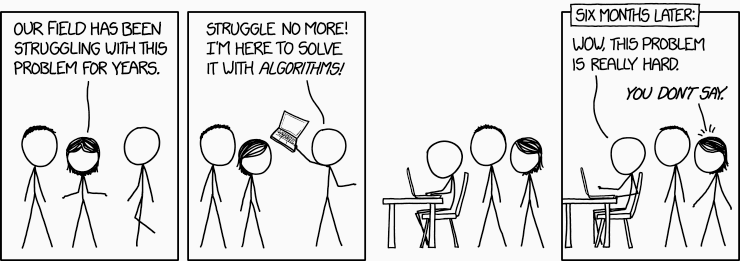
\includegraphics[width=\textwidth]{img/xkcd.png}
%\caption{I can relate to this. [Source: xkcd.com/1831]}
%\end{figure}
%\end{center}
%\end{frame}

%\begin{frame}{Sorry!}
%\begin{large}
%\begin{alertblock}{\large DISCLAIMER}\vspace{.5em}
%In this presentation, we show \textbf{preliminary} results, as this project is still work in progress.
%\end{alertblock}
%\end{large}
%\end{frame}

\begin{frame}{IE Process Pipeline}
\tikzset{%
  materia/.style={draw, text centered, minimum height=1.8em, minimum width=5em, font=\footnotesize},
  etape/.style={materia, fill=blue!20, rounded corners},
  doc/.style={materia, fill=green!20,shape=document, text width=6em, inner ysep=5pt},
  lab/.style={anchor=base,text width=5em,font=\bfseries\itshape\scriptsize},
  back group/.style={fill=yellow!20,rounded corners, draw=black!50, thick, inner ysep=5pt,minimum height=2cm},
  imp/.style={etape}
}
\tikzstyle{myarrows}=[-stealth',line width=.8mm]
\tikzstyle{doublea}=[stealth'-stealth',line width=.3mm]

\tikzset{%
  cascaded/.style = {%
    general shadow = {%
      etape,
      shadow scale = 1,
      shadow xshift = .8ex,
      shadow yshift = .8ex,
      draw},
    general shadow = {%
      etape,
      shadow scale = 1,
      shadow xshift = .4ex,
      shadow yshift = .4ex,
      draw},
    draw}}
    
\pgfdeclarelayer{background}
\pgfdeclarelayer{foreground}
\pgfsetlayers{background,foreground,main}
 
\begin{figure}
\resizebox{\textwidth}{!}{
\begin{tikzpicture}[node distance=1.5em and 3em, align=center]
\node[etape] (token) {Stanford};
\node[etape, right=of token] (lemma) {ClearNLP};
\node[etape, right=of lemma] (pos) {OpenNLP};
\node[etape, right=of pos] (ner) {CoreNLP};
\node[etape, right=of ner] (ie) {UIMA Ruta};

\node[above=of token,lab] (t) {Tokenisation};
\node[above=of lemma,lab] (l) {Lemmatisation};
\node[above=of pos,lab] (p) {POS-Tagging};
\node[above=of ner,lab] (n) {NER};
\node[above=of ie,lab] (i) {Information Extraction};

\begin{pgfonlayer}{foreground}
\node[back group] (start) [fit=(token) (t)]{};
\node[back group] (1) [fit=(lemma) (l)]{};
\node[back group] (2) [fit=(pos) (p)]{};
\node[back group] (3) [fit=(ner) (n)]{};
\node[back group] (end) [fit=(ie) (i)]{};
\end{pgfonlayer}

\node[doc, above=3.5em of start] (doc) {unstructured document};
\node[doc, above=3.5em of end,node distance=2em] (struc) {structured data};

\node[etape, cascaded, below=3em of token] (st) {PosMapper};
\node[etape, cascaded, below=3em of lemma] (sl) {CoreNLP};
\node[etape, cascaded, below=3em of pos] (sp) {MatePos};
\node[etape, cascaded, below=3em of ner] (sn) {OpenNLP};
\node[etape, cascaded, below=3em of ie] (si) {CoreNLP};

\draw[doublea] (token) edge (st);
\draw[doublea] (lemma) edge (sl);
\draw[doublea] (ner) edge (sn);
\draw[doublea] (pos) edge (sp);
\draw[doublea] (ie) edge (si);

%\node[lab,above=0.4em of 3,xshift=-1.6em,align=right,font=\upshape\footnotesize,text width=9em](uima) {UIMA implementation};

%\begin{pgfonlayer}{background}
%\node[dashed,back group, fill=orange!20] [fit=(uima) (start) (1) (2) (3)] {};
%\end{pgfonlayer}

\draw[myarrows] (doc) edge (start) (start) edge (1) (1) edge (2) (2) edge (3) (3) edge (end) (end) edge (struc);
\end{tikzpicture}
}
\caption{IE process pipeline.}
\end{figure}
\end{frame}

\begin{frame}{Named Entity Recognition}
\begin{figure}
\tikzstyle{block} = [rectangle, draw, fill=blue!10, rounded corners, text centered, minimum width=1.5em,font=\footnotesize\ttfamily, node distance=2em]
\begin{tikzpicture}[node distance = .5em, font=\bfseries\large,baseline, text height=1.5ex,text depth=.25ex,highlight/.style={text=orange}]
\node (a) at (0,0) {The};
\node[right=of a,onslide={<2-> highlight}] (b) {quick};
\node[right=of b,onslide={<2-> highlight}] (c) {brown};
\node[right=of c,onslide={<2-> highlight}] (d) {fox};
\node[right=of d] (e) {jump};
\node[right=of e] (f) {over};
\node[right=of f] (g) {the};
\node[right=of g,onslide={<2-> highlight}] (h) {lazy};
\node[right=of h,onslide={<2-> highlight}] (i) {dog};
\node[right=of i] (j) {.};

\node[block,fill=Fuchsia!30,below of=a] {DT};
\node[block,fill=yellow!30,below of=b] {JJ};
\node[block,fill=yellow!30,below of=c] {JJ};
\node[block,fill=RoyalBlue!30,below of=d] {NN};
\node[block,fill=green!30,below of=e] {VBD};
\node[block,fill=orange!30,below of=f] {IN};
\node[block,fill=Fuchsia!30,below of=g] {DT};
\node[block,fill=yellow!30,below of=h] {JJ};
\node[block,fill=RoyalBlue!30,below of=i] {NN};
\node[block,fill=gray!30,below of=j] {.};

\node at (0,-1.5) {};
\node[above of=e,gray,node distance=1.3em,font=\mdseries] {\footnotesize jumps}; 
\end{tikzpicture}
\caption{POS-tagging examples after lemmatisation.}
\end{figure}
\end{frame}

\begin{frame}[fragile]{Adapting the NER}\large
Most NERs (e.\,g.\ \textbf{Stanford CoreNLP}) only recognise 8 entities types:

\begin{center}\ttfamily
\begin{tabular}{lp{4em}l}
PERSON&&DATE\\
ORGANIZATION&&TIME\\
LOCATION&&MONEY\\
PERCENT&&MISC
\end{tabular}
\end{center}

So we have to add the \alert{custom entity type \texttt{FORM}}.
\end{frame}

\begin{frame}{Two approaches for NER}
\begin{minipage}[t]{0.45\textwidth}
\textbf{Rule-based approach}
\begin{itemize}
\item High precision, but lower recall

$\Rightarrow$ \alert{Many many rules?!}
\end{itemize}
\visible<2->{
\begin{figure}
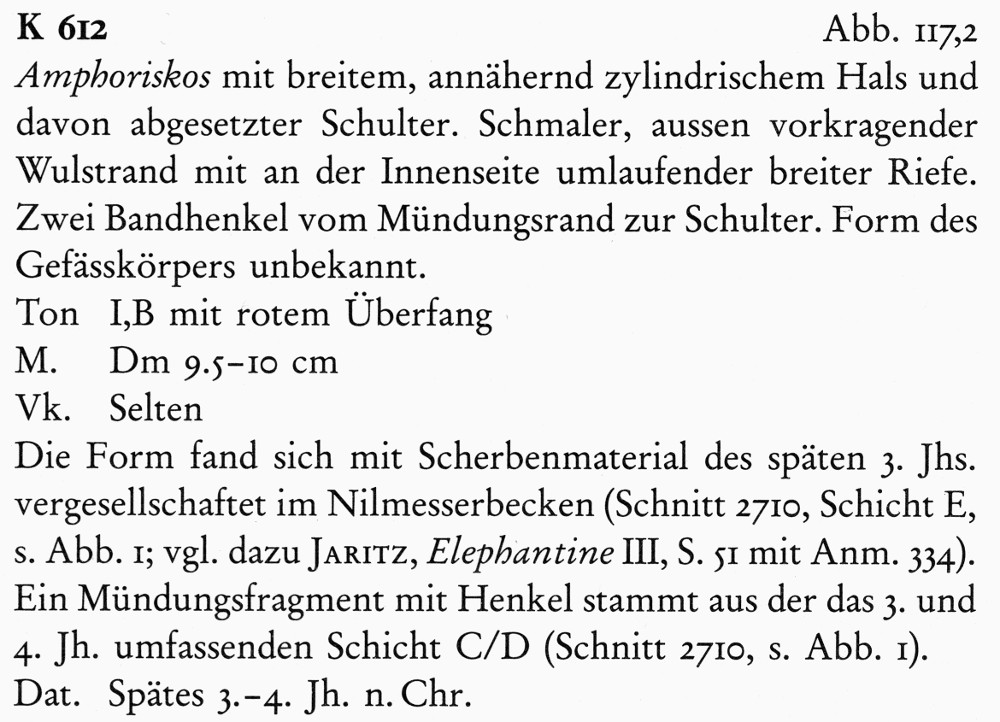
\includegraphics[width=\textwidth]{img/eleph.jpg}
\caption{Excerpt from \cite{eleph}.}
\end{figure}}
\end{minipage}\pause\pause\hfill
\begin{minipage}[t]{0.45\textwidth}
\textbf{Machine-learning approach}
\begin{itemize}
\item Lower precision, but high recall
\item \alert{Needs to be trained!}
\end{itemize}%\vspace*{-1em}
\visible<4>{
\begin{figure}
\hspace*{-1em}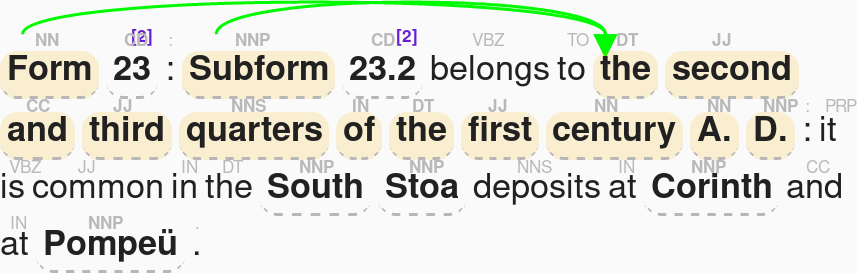
\includegraphics[width=1.05\textwidth]{img/iepy.png}
\caption{Manually annotated sentence from \cite{consp} in \texttt{iepy}.}
\end{figure}
}
\end{minipage}
\end{frame}

\begin{frame}{Temporal Expressions}
With \textbf{\textit{\textsc{HeidelTime}}} temporal expressions are mapped to TIMEX3 standard
\begin{center}
{\renewcommand{\arraystretch}{1.2}%
\begin{tabular}{rcl}
\texttt{around 140 B.\,C.}&$\longmapsto$&\texttt{APPROX BC0140}\\
\texttt{Spätes 3.–4.\ Jh.\ n.\,Chr.}&$\longmapsto$&\texttt{END 02};~~ \texttt{03}\\
\texttt{second quarter first century B.\,C.}&$\longmapsto$&\texttt{XXXX-Q2 BC00}\\
\texttt{first half third century A.\,D.}&$\longmapsto$&\texttt{XXXX-H1 02}\\
\end{tabular}
}
\end{center}

\textbf{\textsc{HeidelTime}} supports many other languages, e.\,g.\ German, Italian, French, \dots
\end{frame}

\begin{frame}[fragile]{Relation Extraction}
\begin{center}
\begin{tabularx}{\textwidth}{CCC}
\toprule
\textbf{Subject}&\textbf{Relation}&\textbf{Object}\\\midrule
quick brown fox&jump over&lazy dog\\
K 612&dates&\texttt{03}\footnote{\enquote{4th century A.\,D.}}\\
Subform 23.2&occurs&North Italy\\
Subform 23.2&dates&\texttt{XXXX-Q2 00}\footnote{\enquote{second and third quarters of the first century A.\,D.}}\\
\bottomrule
\end{tabularx}\bigskip\pause

\begin{minipage}{0.3\textwidth}\flushright
\textbf{$\boldsymbol{\Rightarrow}$ e.\,g.}
\end{minipage}\hfill
\begin{minipage}{0.65\textwidth}
{
\begin{verbatim}
{  "form":   "23.2",
   "dating": "XXXX-Q2 00"  }
\end{verbatim}
}
\end{minipage}
\end{center}
\end{frame}

%NOTE: supports Pleiades and GeoNames

%\begin{frame}{Locations with \textsc{HeidelPlace}}
%\begin{figure}
%\hspace*{-1em}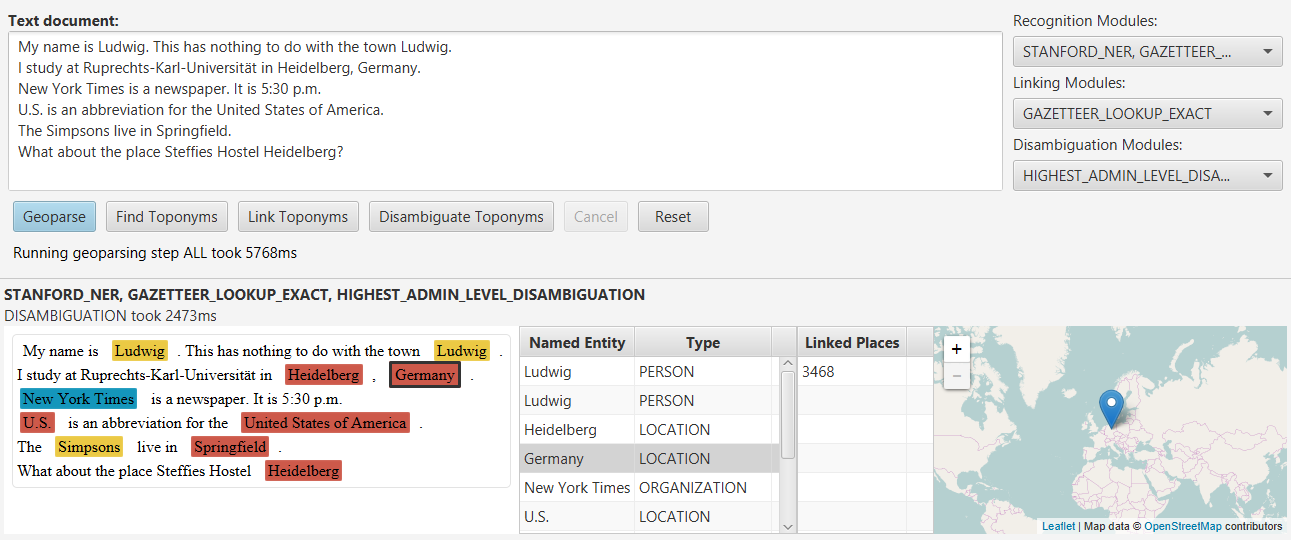
\includegraphics[width=1.025\textwidth]{img/heidelplace.png}
%\caption{Screenshot of \textsc{HeidelPlace}.}
%\end{figure}
%\end{frame}

\section{Multilingualism}

\begin{frame}{Background}
Two problems:
\begin{itemize}
\item Linguistic
\item Conceptual
\end{itemize}
\end{frame}

\begin{frame}{Different languages}
\begin{center}
\begin{figure}
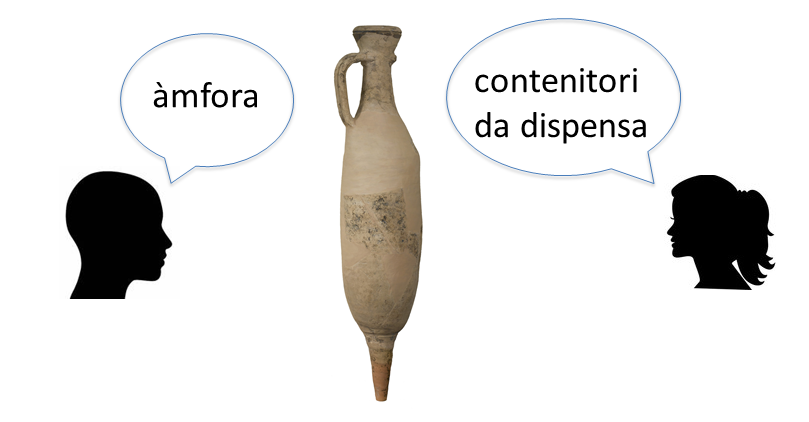
\includegraphics[width=\textwidth]{img/tim_vocab_1.png}
\end{figure}
\end{center}
\end{frame}

\begin{frame}{Different traditions}
\begin{center}
\begin{figure}
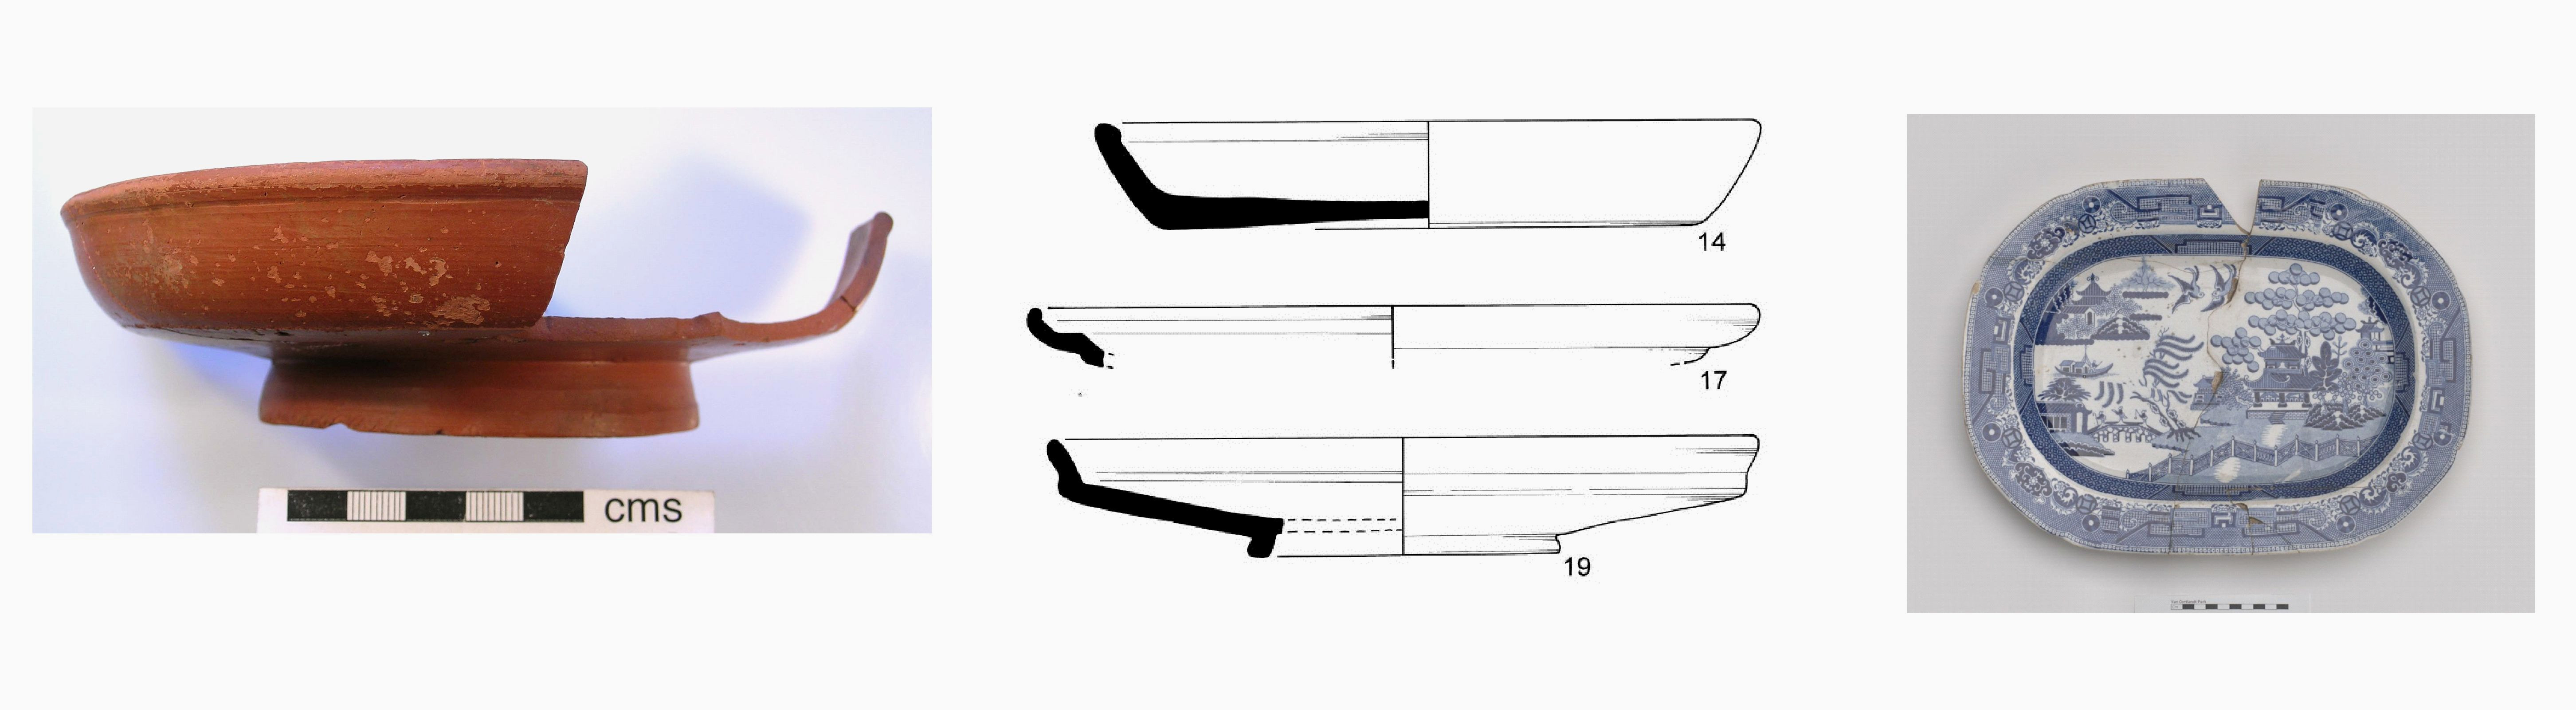
\includegraphics[width=\textwidth]{img/tim_plate_platter_dish.jpg}
\caption{Plate, platter or dish?}
\end{figure}
\end{center}
\end{frame}

\begin{frame}{Creating controlled vocabularies}
Creating wordlists that project team would be most useful to describe the key features of a vessel or sherd
\begin{itemize}
\item Sherd type (e.g. rim or handle)
\item Form (e.g. plate or bowl)
\item Decoration form (e.g. burnished)
\item Decoration color (e.g. yellow)
\item Fabric (e.g. Dressel 28 fabric)
\end{itemize}
\end{frame}

\begin{frame}{Lessons from ARIADNE}
\hfill\raisebox{-.9em}{
\includegraphics[width=4cm]{img/tim_ariadne_logo.png}}\newline
Used tools and methodology developed for the ARIADNE project by the Hypermedia Research Group at the University of South Wales \newline
\begin{itemize}
\item Created a neutral spine based on the Getty Institute's Art and Architecture Thesaurus (AAT)
\item This spine was populated by members from partner organisations, identifying common terms and concepts within it
\item Project partners then mapped terms in their language to this neutral spine
\item French terms supplied courtesy of a 2001 Masters thesis by Caroline \textsc{Sourzat} (thanks to Eleni Schindler Kaudelka for identifying this on the ArchAIDE blog!)
\end{itemize}
\end{frame}

\begin{frame}{Mapping terms and concepts (part 1)}
Often this was very straightforward, for example:
\begin{itemize}
\item The Italian terms \emph{graffita, graffita a punta, graffita a stecca} = \enquote{sgraffito} (http://vocab.getty.edu/aat/300266416)
\item The Spanish term \emph{Cántaro} = \enquote{jars} (http://vocab.getty.edu/aat/300195348)
\item The German terms \emph{gebogener Henkel, Ohrförmiger Henkel, langer Vertikalhenkel} = \enquote{handles} (http://vocab.getty.edu/aat/300266416)
\end{itemize}
\end{frame}

\begin{frame}{Mapping terms and concepts (part 2)}
Often this was more complicated, with partners having differing perceptions on what to call something (e.g. \enquote{plate} versus \enquote{platter})\newline
\newline
In truth, this confusion may also be reflected by what has come out of the ground!\newline
\newline
An advantage of using the AAT (a \enquote{SKOS'd} thesaurus), is that ambiguity or difference in nomenclature can be resolved by  a broader term or concept, so for example \dots
\end{frame}

\begin{frame}{Mapping terms and concepts (part 3)}
Looking at the hierarchies for plate and platter in the AAT we can see that both are \enquote{dishes (vessels for food)}, or even broader \enquote{culinary containers}. So whole we can retain our original classifications (and this is essential for text mining), we can agree at a fundamental level \emph{what these fundamentally are}
\begin{center}
\begin{figure}
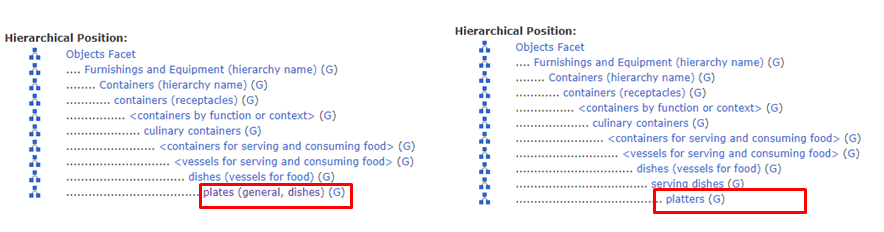
\includegraphics[width=\textwidth]{img/tim_hierarchy_plate.png}
\caption{AAT Hierarchies for Plate and Platter}
\end{figure}
\end{center}
\end{frame}

\begin{frame}{Outlook}
\begin{itemize}
\item Recognize reigns of emperors as \texttt{DATE} entities
\item Coreferences in general
\item \textsc{HeidelTime}:

second and \textbf{third quarter} of the \textbf{first century A.\,D.}\quad$\longmapsto$\quad\texttt{XXXX-Q3};~~\texttt{00}
\item Returning to difference in ceramic recording details
\item Fabric names often contain locations, e.\,g.\ \emph{Magdalensberg xyz}
\item Location sometimes narrow, sometimes whole regions
\item In many cases the form is not named in particular but just described
\end{itemize}
\end{frame}

\begin{frame}{References}

\printbibliography[heading=none]
\end{frame}


\begin{frame}[plain]
\vfill\vfill\vfill
\begin{center}\Large
Thank you very much for your attention!\\\bigskip

Questions?
\end{center}\vfill\vfill

\hfill
\begin{minipage}{0.7\textwidth}\scriptsize
\begin{flushright}
This project has received funding from the European Union's Horizon 2020 research and innovation programme under grant agreement \textnumero\ 693548
\end{flushright}
\end{minipage}\hspace*{1em}
\begin{minipage}{0.1\textwidth}

\includegraphics[width=\textwidth]{img/eu_flag.ps}
\end{minipage}
\end{frame}

\maketitle

\end{document}
